\chapter{Education}
\label{chap:education}

\inspirationalquote{Knowing the students might one day
%find a way to
fix their concurrency bugs...
it fills you with determination.}{Undertale (paraphrased)}

Concurrency is taught in as many different ways as there are
systems programming classes at universities which teach the subject.
Yet one thing they all have in common is presenting the concurrency bug
as some elusive menace,
against which humanity's best weapon is mere random stress testing.
This chapter will prove stateless model checking's mettle as a better alternative in the educational theatre.

While the previous chapter demonstrated Landslide's bug-finding power
compared to prior MC techniques in a controlled environment,
whether it offers pedagogical merit in the hands of students and/or TAs is a separate question.
And while my M.S. thesis~\cite{landslide} showed that students
could annotate P3 Pebbles kernels and thence use Landslide to debug them,
the annotations alone required 2 hours of effort on average per user,
meaning the only students who could benefit were the ones already succeeding enough to have such free time.
Since then, I have extended Landslide with a fully-automatic instrumentation process
for Pebbles thread libraries (P2s) (\sect{\ref{sec:education-pebbles-instrumentation}})
and Pintos kernels (\sect{\ref{sec:education-pintos-instrumentation}})
to improve its accessibility.

I have run several user studies in the Operating Systems classes
at Carnegie Mellon University (CMU), University of Chicago (U. Chicago),
and \revisionminor{The Pennsylvania} State University (PSU),
wherein students get to use Landslide to find and diagnose their own bugs during the semester.
At CMU, I analyzed logs and code snapshots taken as students used Landslide during P2
(\sect{\ref{sec:education-eval-bugfinding}}),
as well as the grades ultimately assigned after students who either did or didn't use Landslide submitted their projects
(\sect{\ref{sec:education-eval-grades}}).
At CMU and PSU, I surveyed students on their experience after submitting their Landslide-debugged P2s
(\sect{\ref{sec:education-eval-survey}}).
At U. Chicago, I collaborated with a TA to check submitted Pintos kernels,
then \revisionminor{they} returned any resulting bug reports to students
(\sect{\ref{sec:education-eval-bugfinding}})
and likewise surveyed them on the quality of the diagnostic output
(\sect{\ref{sec:education-eval-survey}}).

%%%%%%%%%%%%%%%%%%%%%%%%%%%%%%%%%%%%%%%%%%%%%%%%%%%%%%%%%%%%%%%%%%%%%%%%%%%%%%%%

\section{Pebbles}

This section presents the user studies done in
%CMU's 15-410 and PSU's \psuos classes,
%in semesters Fall 2015 to Spring 2018 and in Spring 2018 alone, respectively,
%taught by David A. Eckhardt and Timothy Zhu, respectively.
CMU's 15-410 in semesters Fall 2015 to Spring 2018,
taught by David A. Eckhardt,
and in PSU's \psuos in Spring 2018,
taught by Timothy Zhu.
In both cases the instructors assisted to introduce me during the guest lecture
%(see below)
and to distribute the recruiting emails;
TAs were not involved.
The in-house user study has CMU IRB approval under study number STUDY2016\_00000425,
and the external user study under STUDY2017\_00000429.

% Possible experiment questions
% compare e.g. use after free bug reporce from OOPSLA data set, to P2 grade files, see who has thread exit uafs
% is landslide better at finding thread uafs than TAs
% same Q for other stuff.. (expect paraguay answer to be "no", explain why)

\subsection{Recruiting}
\label{sec:education-pebbles-recruiting}

Since the Spring 2015 semester I have given a guest lecture in 15-410
to recruit students to participate in the user study.
The 50-minute lecture is given 1 week into the 2.5-week-long P2 project,
approximately when the students should be getting child threads running in {\tt thr\_create()}
and experiencing concurrency bugs for the first time.
It introduces the research subject abstractly
using an example ``Paradise Lost'' bug from a previous lecture \cite{paradise-lost},
explains how Landslide works concretely,
shows a short demo of effortlessly using Landslide to find the example bug,
and provides the necessary IRB legalese about the risks and benefits of participation.
The most recent lecture slides are available on the course website at
\url{http://www.cs.cmu.edu/~410-s18/lectures/L14_Landslide.pdf},
and all semesters' editions at
\url{https://github.com/bblum/talks/tree/master/landslide-lecture}.

The PSU version of the lecture
%was given in Spring 2018, and
is available at
\url{http://www.contrib.andrew.cmu.edu/~bblum/psu-lecture.pdf}
as well as under the github link above.
Being a 70-minute lecture slot rather than 50, I extended the demo to
both find and (attempt to) verify a fix for two bugs:
one a simple data race and the other the more complicated Paradise Lost bug as above.
After finding each bug, I demonstrated using Landslide on a fixed version of the code
to show how it proves the test case correct by completing all state spaces,
or (in the case of Paradise Lost) suffers an exponentially-exploding state space.
%Not that I scientifically measured it or anything,
This extended demo seemed to help students more clearly understand Landslide's intended workflow,
at the cost of about 10-15 extra minutes of lecture time
\revisionminor{(of course, this is an anecdotal opinion, not a scientific conclusion).}

At both schools students then signed up using a Google form I emailed them,
which upon completion linked them to the Landslide user guide,
which is available at
\url{http://www.contrib.andrew.cmu.edu/~bblum/landslide-guide-p2.pdf}
(CMU version)
and
\url{http://www.contrib.andrew.cmu.edu/~bblum/landslide-guide-psu.pdf}
(PSU version)
and
\url{https://github.com/bblum/talks/tree/master/irb}
(both versions).

During the last week of P2 at CMU, I held several ``Landslide clinic'' sessions
(basically office hours, but given a different name to remind students
to limit themselves to questions a normal TA couldn't answer),
where students could receive in-person technical and/or moral support.
Collecting study information during these sessions was not included in the IRB protocol.
In the PSU study, I had returned to Pittsburgh shortly after giving the lecture,
so technical support for PSU students was limited to email correspondence.

\subsection{Automatic instrumentation}
\label{sec:education-pebbles-instrumentation}

As described in \sect{\ref{sec:landslide-setup}},
all setup from the user's point of view is handled through the {\tt p2-setup.sh} script.%
\footnote{PSU's version is called {\tt psu-setup.sh};
in this section {\tt p2-setup.sh} refers to both unless otherwise noted.
}
It, its helper scripts (\sect{\ref{sec:landslide-glue}}),
and the {\tt landslide} script itself contain several checks to prevent
studence
from accidentally misusing Landslide in ways that could produce mysterious crashes, false bug reports, and so on
(the need for each \revisionminor{check}, as the reader might imagine, discovered through bitter experience).
These include:
\begin{itemize}
	\item {\tt p2-setup.sh} checks if the directory argument correctly points at the top-level P2 basecode directory
		rather than any subdirectories such as {\tt user/libthread/}.
	\item {\tt check-need-p2-setup-again.sh} checks if any source files in the original P2 source directory
		(the argument supplied to {\tt p2-setup.sh}) \revisionminor{have been updated},
		in case the student hoped to fix some bug and verify their fix but forgot to re-run the setup script.
	\item {\tt landslide} checks the supplied test name matches one of the endorsed Landslide-friendly tests
		(students love trying to run Landslide with {\tt racer}, {\tt largetest},
		or even the string {\tt OPTIONS}).
	\item {\tt landslide} checks if any other instance of itself is simultaneously running in the same directory,
		and if so, refuses to do so and advises the student
		to {\tt git clone} the repository afresh for simultaneous use.%
		\footnote{This is ironically implemented with a non-atomic lock file
		and should really be using {\tt flock} instead.
		}
\end{itemize}
\vspace{1em}

\noindent Landslide also includes several P2-specific instrumentations and features to cope with various student irregularities:
\begin{itemize}
	\item Quicksand emits different combinations of {\tt within\_function}/{\tt without\_function} directives
		for Landslide depending on the name of the test.
		For example, for {\tt paradise\_\allowbreak{}lost},
		\revisionminor{designed to test student semaphore code,}
		Landslide will not preempt in a function named {\tt critical\_section()},
		which the test case uses to protect an internal counter used to detect the bug;
		and it will not preempt in any of the {\tt thr\_*()} thread library API functions
		for tests intended to target just the concurrency primitives.
		In future work this could be improved as annotations to be placed inside the test case code itself.
	\item Landslide finds ad-hoc synchronization patterns,
		such as {\tt while (!flag) yield()} or {\tt while (xchg(...)) continue},
		which students often open-code rather than using the prescribed synchronization API,
		and treats them as synchronization points as described in \sect{\ref{sec:landslide-blocking}}.
	\item Landslide finds ``too suspicious'' spinwait-loops in mutex implementations
		which are neither yield- nor {\tt xchg}-loops (as described above),
		which would ordinarily be classified as infinite loop bugs,
		and reports them with a suggestive message ({\tt undesirable\_\allowbreak{}loop\_html()} in {\tt landslide.c})
		referring the student to the appropriate lecture material
		\cite{synchronization-2}.
	\item The {\tt landslide} wrapper script logs the time and command-line options of invocation
		and captures a snapshot of the student code and results of the test and saves them to AFS
		\revisionminor{(CMU's network file system)~\cite{afs}}
		after each run.
		% HURDLE_VIOLATION -- no, this is for p3 (context switcher) features only
\end{itemize}

\subsection{Test cases}
\label{sec:education-pebbles-tests}

Landslide ships with several ``approved'' test cases,
i.e., programs copied from, derived from, or at least vaguely resembling
the tests distributed with P2,
which I curated to produce concurrent behaviour suitable for stateless model checking.
Some tests are crafted to target specific bugs which,
from personal experience as a TA, are common in many student submissions;
others are crafted to exercise generally concurrency-heavy code paths and uncover any number of unforeseen problems.
Many use some of the features/annotations described in \sect{\ref{sec:landslide-testcases}}.

%\subsubsection{Test case list}

The following tests were released to CMU students:
\begin{itemize}
	\item {\tt broadcast\_test}:
		Tests the {\tt cond\_broadcast()} signalling path with a single waiter.
	\item {\tt mutex\_test}:
		Tests student mutexes under 2 threads with 2 iterations
		(the \revisionminor{second} iteration serves to expose problems with {\tt mutex\_unlock()} as well as {\tt mutex\_lock()}).
		This test uses the {\tt TESTING\_MUTEXES}
		described in \sect{\ref{sec:landslide-staticconfig}}
		to enable data-race preemption points within the mutex implementation.
	\item {\tt paradise\_lost}:
		Written for the sake of the Landslide lecture demo
		(\sect{\ref{sec:education-pebbles-recruiting}}).
		Tests for the Paradise Lost bug by attempting to break mutual exclusion.
	\item {\tt paraguay}:
		Copied directly from the P2 test suite;
		tests for proper handling of seemingly ``spurious'' wakeups in {\tt cond\_wait()}.
		Written by Michael J. Sullivan.
	\item {\tt rwlock\_downgrade\_read\_test}:
		Copied directly from the P2 test suite;
		tests for mutually-exclusive and deadlock-free {\tt rwlock\_downgrade()}
		\revisionminor{(a function which atomically converts a lock held in exclusive write mode to shared read mode)}.
		Written by me (as a TA).
	\item {\tt thr\_exit\_join}:
		Copied directly from the P2 test suite;
		tests for a variety of problems between {\tt thr\_exit()} and {\tt thr\_join()},
		but especially for memory issues pertaining to stack deallocation.
\end{itemize}
\vspace{1em}

\noindent The following tests were released to PSU students, in addition to the ones above:
\begin{itemize}
	\item {\tt atomic\_compare\_swap}:
		Tests the {\tt cmpxchg} assembly function for being properly atomic.
		Uses the {\tt magic\_*} global variables described below, and invokes {\tt vanish()} directly,
		to avoid requiring the student to implement {\tt thr\_join()}/{\tt thr\_exit()}
		before being able to run this test.
	\item {\tt atomic\_exchange}:
		As above for {\tt xchg}.
	\item {\tt atomic\_fetch\_add}:
		As above for {\tt xadd}.
	\item {\tt atomic\_fetch\_sub}:
		As above for {\tt xadd}.
	\item {\tt broadcast\_two\_waiters}:
		As {\tt broadcast\_test}, but uses two waiting threads to ensure both get signalled.
\end{itemize}
\vspace{1em}

\noindent The tests can all be viewed at \url{https://github.com/bblum/landslide/tree/master/pebsim/p2-basecode/410user/progs}.

\subsection{Survey}
\label{sec:education-survey-pebbles}

Starting in Fall 2017, I sought to gauge the students' personal opinions on their experience with Landslide,
in addition to simply counting
from the automatic snapshots
how many bugs were found.
Shortly after the P2 submission deadline,
I asked participants to answer several survey questions, reproduced below.
%distributed via email as a Google Doc.

\begin{enumerate}
	\item How many bugs did Landslide help you find in your code? (Please indicate a number.)
	\item How many of the bugs you found with Landslide do you believe you fixed before submitting your project? (You may answer ``all'', ``none'', or a number.)
	\item How many of the bugs you found with Landslide did you verify you had fixed by running Landslide again to make sure the bug was gone? (You may answer ``all'', ``none'', or a number.)
	\item In addition to the bugs Landslide found, did it report anything that you believe was NOT a bug? For example, Landslide printed an execution trace that was actually impossible, or Landlside reported a bug about some behaviour that was actually allowed by the P2 specification. (If so, please describe.)
	\item I found Landslide's debugging output easy to understand.
		(Multiple choice from strongly disagree to strongly agree.)
	\item It's easier to diagnose the root cause of a bug with Landslide than with a stress test (e.g. juggle).
		(Multiple choice from strongly disagree to strongly agree; plus ``Not sure'' and ``Easier for some bugs but harder for others'')
	\item I felt the time I saved by having Landslide to help debug was worth the time it took me to learn how to use Landslide.
		(Multiple choice from strongly disagree to strongly agree.)
	\item I feel that by using Landslide I learned to understand concurrency better.
		(Multiple choice from strongly disagree to strongly agree.)
	\item Suppose after you submitted your project, % "P2" for cmu, "project" for pintos
		we gave you 100 CPU-hours on the cloud provider of your choice to test it. Then we extended the project deadline by a day for you to use the results to fix bugs and get partial credit. How would you divide that CPU time between the staff-provided stress tests and Landslide?
		(Multiple choice: 0/10/.../100 CPU-hours on Landslide, 100/90/.../0 CPU-hours on stress tests.)
	\item If I found out next semester that a friend of mine (or a student in my degree program) were taking OS, I would recommend that they should probably invest some time during the project % "P2" for cmu, as above
		to learn Landslide and try to find bugs with it.
		(Multiple choice from strongly disagree to strongly agree.)
	\item Regarding the previous question, why or why not?
\suspend{enumerate}
\vspace{1em}

\noindent The following questions were served only on the CMU version of the survey.
\resume{enumerate}
	\item Did you answer this survey together with your partner, or on your own while they were busy? (If you both have time for it, please try to submit one survey together.)
		(Multiple choice: together or alone)
	\item Your andrew ID
	\item Your partner's andrew ID (if any)
\suspend{enumerate}
\vspace{1em}

\noindent The following questions were served only on the PSU version of the survey.
\resume{enumerate}
	\item Any feedback on how Landslide's user interface could be improved / made easier to use or understand? (setup process, messages printed while running, or the execution trace / stack traces emitted after a bug is found?)
	\item Your PSU username
\end{enumerate}

%%%%%%%%%%%%%%%%%%%%%%%%%%%%%%%%%%%%%%%%%%%%%%%%%%%%%%%%%%%%%%%%%%%%%%%%%%%%%%%%

\section{Pintos}

This section presents the user study done in U. Chicago's \uchos class in the Fall 2017 semester,
taught by Haryadi Gunawi.
Kevin Zhao, the TA, assisted to run Landslide on student submissions
and to distribute recruiting materials and testing results.
The study has CMU IRB approval under study number STUDY2017\_00000429.

\subsection{Recruiting}

For this study students were recruited remotely via email.
After each of the {\em threads} and {\em userprog} project deadlines (\sect{\ref{sec:overview-pintos}}),
\uchos staff sent students an email inviting them to volunteer to receive Landslide's bug reports,
disclaiming that it did not represent part of the official grading process but could help improve their future submissions.

\subsection{Automatic instrumentation}
\label{sec:education-pintos-instrumentation}

As described in \sect{\ref{sec:landslide-setup}},
all setup from the user's point of view is handled through the {\tt pintos-setup.sh} script.
It
and its helper {\tt pebsim/pintos/import-pintos.sh}
perform most of the same sanity checks as listed in \sect{\ref{sec:education-pebbles-instrumentation}},
then applies the patch {\tt annotate-\allowbreak{}pintos.patch}
(plus several more hacks in the script itself)
to insert the {\tt tell\_landslide()} annotations (\sect{\ref{sec:tell-landslide}})
into the student's kernel code.
The following tricks were developed after trial-and-error on student submissions from the same semester,
and serve to make sure the annotations apply consistently
to (almost) all variations of commonly-submitted code.

\begin{itemize}
	\item Finds the declaration of {\tt ready\_list}, the scheduler runqueue declared by the basecode,
		%and detects if the student has modified to be an array of lists rather than a single one.
		\revisionminor{and detects if the student has replaced the default definition
		with a different name and/or data structure.}
		If so,
		%defines the length of that array in a macro to be used by {\tt is\_runqueue()}
		\revisionminor{emits macros to configure {\tt is\_runqueue()}'s behaviour to handle
		certain common alternate approaches}
		(part of the patch described below).
		Either way defines a function {\tt get\_rq\_addr()} to return the address of the %(first)
		list.
	\item Changes the basecode's definition of {\tt TIME\_SLICE} from 4 to 1 (units of timer ticks)
		so Landslide's timer injection will properly drive the context switcher.
	\item Inserts {\tt tell\_landslide\_forking()} into {\tt thread.c}
		(using {\tt sed} rather than the patch, described below,
		because it must go in a function which students have to implement,
		which is likely to disturb the context and make a patch fail).
	\item Adds the new {\tt priority-donate-multiple} test.
	\item Applies the {\tt annotate-pintos.patch} patch to the imported student implementation, which:
	\begin{itemize}
		\item Adds {\tt tell\_landslide\_thread\_on\_rq()}
			and {\tt tell\_landslide\_thread\_off\_rq()}
			annotations
			to {\tt list\_insert()} and {\tt list\_remove()} respectively
			(in {\tt lib/kernel/\allowbreak{}list.c}, which the students don't modify),
			which
			check whether the argument list
			is the scheduler runqueue
			using a helper function {\tt is\_runqueue},
			which in turn uses {\tt get\_rq\_addr()} and {\tt READY\_LIST\_LENGTH} described above.
		\item Modifies the existing {\tt priority-sema} and {\tt alarm-simultaneous} tests to be more Landslide-friendly.
		\item Inserts the {\tt tell\_landslide\_sched\_init\_done()},
			{\tt tell\_landslide\_vanishing()},
			and {\tt tell\_landslide\_thread\_switch()}
			annotations in the appropriate places
			(which the students generally do not modify).
	\end{itemize}
	\item Detects if the student has renamed the {\tt elem} field of the TCB struct,
		and if so renames its use in {\tt is\_runqueue()} (described above) correspondingly.
	\item Detects if the student has renamed the {\tt cur} (currently running thread) variable
		in the context switcher, and if so renames it back.
\end{itemize}

\subsection{Test cases}
\label{sec:education-pintos-tests}

Like the P2 tests, the Pintos test cases are either hand-picked from the provided unit tests,
with an eye for which will produce interesting concurrent behaviour,
or created using a TA's intuition for the most likely student bugs.
The following tests are approved to be Landslide-friendly:

\begin{itemize}
	\item {\tt priority-sema}:
		Modified to be Landslide-friendly from the basecode, for {\em threads}.
		Creates two child threads to wait on a semaphore and signals them.
		Replaces threads with different priorities
		(originally chosen to produce deterministic output which the test checked for)
		with threads of the same priority.
	\item {\tt alarm-simultaneous}:
		Modified to be Landslide-friendly from the basecode, for {\em threads}.
		Creates two child threads which each invoke {\tt timer\_sleep()} for a different amount of time.
		Number of (threads,iterations) reduced from (3,5) to (2,1).
	\item {\tt wait-simple}:
		Unmodified from the basecode's version, for {\em userprog}.
		Userspace process {\tt exec()}s a child process, which immediately exits, and {\tt wait()}s on it.
	\item {\tt wait-twice}:
		Unmodified from the basecode's version, for {\em userprog}.
		Slightly more complicated version of {\tt wait-simple},
		intended to expose failure-path bugs if the former finds no easier ones.
	\item {\tt priority-donate-multiple}:
		Written by Kevin Zhao, TA at U. Chicago, for {\em threads}.
		Tests for a priority donation race during {\tt lock\_release()}
		in which a thread holding a lock can accidentally keep a contending thread's donated priority
		after finishing releasing it.
\end{itemize}
\vspace{1em}

The (unpatched versions of) the first four tests are available at
\url{https://github.com/bblum/pintos} (a fork of the main Pintos basecode repository).
%\url{https://github.com/Berkeley-CS162/group0/tree/master/pintos/src/tests}.
The fifth test is available at
\url{https://github.com/bblum/landslide/blob/master/pebsim/pintos/priority-donate-multiple.c}.

\subsection{Survey}
\label{sec:education-survey-pintos}

Similar to the survey for Pebbles projects
\sect{\ref{sec:education-survey-pebbles}},
I surveyed the Pintos user study participants for their opinions.
Because of the different nature of the user study, of course,
the questions here focus more on the debugging experience than on using Landslide directly.

\begin{enumerate}
	\item How many Landslide bug reports did you receive from course staff? (Please indicate a number.)
	\item Among those bug reports, how many were you able to diagnose and recognize the root cause in your code? (You may answer ``all'', ``none'', or a number.)
	\item Among those bug reports, how many described a behaviour that you believe was NOT a bug? For example, Landslide printed an execution trace that was actually impossible, or Landslide reported a bug about some behaviour that was actually allowed by the Pintos specification. (You may answer ``all'', ``none'', or a number.)
	\item About how much time did you spend interpreting Landslide's debugging output? (Please indicate a number of minutes, or a range if uncertain, e.g. ``30-60 minutes''.)
	\item I found Landslide's debugging output easy to understand.
		(Multiple choice from strongly disagree to strongly agree.)
	\item It's easier to diagnose the root cause of a bug with Landslide than with a stress test (for example {\tt exec-multiple}).
		(Multiple choice from strongly disagree to strongly agree; plus ``Not sure'' and ``Easier for some bugs but harder for others'')
	\item I feel that by interpreting Landslide's debugging output I learned to understand concurrency better.
		(Multiple choice from strongly disagree to strongly agree.)
	\item These kinds of concurrency bugs are important to fix, even though they don't count against my grade.
		(Multiple choice from strongly disagree to strongly agree.)
	\item Suppose after you submitted your pintos, we gave you 100 CPU-hours on the cloud provider of your choice to test it. Then we extended the project deadline by a day for you to use the results to fix bugs and get partial credit. How would you divide that CPU time between the staff-provided stress tests and Landslide?
		(Multiple choice: 0/10/.../100 CPU-hours on Landslide, 100/90/.../0 CPU-hours on stress tests.)
	\item If course staff were to allow students to resubmit updated code after reviewing Landslide bug reports to receive partial credit for each bug that had been fixed, it would be worth my time to try that (even if I could be spending that time working on the next project instead).
		(Multiple choice from strongly disagree to strongly agree.)
	\item If a friend of mine took OS next semester, I would recommend that they should sign up to receive Landslide bug reports during projects in the future.
		(Multiple choice from strongly disagree to strongly agree.)
	\item Regarding the previous question, why or why not?
	\item Your name.
	\item Your project partner's name (if applicable)
\end{enumerate}

%%%%%%%%%%%%%%%%%%%%%%%%%%%%%%%%%%%%%%%%%%%%%%%%%%%%%%%%%%%%%%%%%%%%%%%%%%%%%%%%

\section{Evaluation}

I pose the following evaluation questions.

\begin{itemize}
	\item How many bugs, and of what severities, does Landslide help students find and fix before submitting their code?
	\item Does Landslide use result in higher quality submissions, whether directly for P2, or for subsequent projects as well?
	\item Do students feel the experience is worthwhile, as compared to stress testing?
	\item How well does Landslide apply to operating systems projects outside of CMU?
\end{itemize}
\vspace{1em}

The data set \revisionminor{comprises} Landslide's automatically-generated usage snapshots
from CMU students from semesters Spring 2015 to Spring 2018 inclusive,
% and PSU \psuos from Spring 2018, % no snapshots from psu
CMU's official project grades from same,
CMU students' survey responses and submitted project code from Fall 2017 and Spring 2018,
PSU students' survey responses and submitted project code from Spring 2018,
and U. Chicago students' survey responses from Fall 2017.
Table~\ref{tab:photo-of-ze-studence} shows the student participation rate across semesters
for the thread library study.%
\footnote{
Participation at CMU was determined by receiving any automatic usage snapshots;
participation at PSU was determined, for lack of snapshots, by sign-up form submissions, which might over-count slightly.
}
% and PSU

\begin{table}[h]
	\begin{center}
		% ugh this looks so stupid
		% but better than latex's output looking stupid
		\begin{tabular}{r|crcrc|r}
			& \multicolumn{5}{c|}{\bf Used Landslide?} & \\
			\bf Semester & & \bf yes & & \bf no & & \bf Total \\
			\hline
			% group-[redacted] had a p2/ dir, but not in grade files
			CMU S'15	& &   8	& &  18	& &  26 \\
			CMU F'15	& &  22	& &   8	& &  30 \\
			CMU S'16	& &  18	& &  16	& &  34 \\
			CMU F'16	& &  12	& &   6	& &  18 \\
			CMU S'17	& &  19	& &  13	& &  32 \\
			CMU F'17	& &  14	& &   5	& &  19 \\
			CMU S'18	& &  10	& &   8	& &  18 \\
			\hline
			U. Chicago F'17	& &   4	& &  17	& &  21 \\ % 21 taken from number of submitted 'threads', idk abt userprog
			PSU S'18	& &  38	& &  98	& & 136 \\
			\hline
			\bf CMU total	& & 103	& &  74	& & 177 \\
			\bf Non-CMU total
					& &  42	& & 115	& & 157 \\
			\bf Total	& & 145	& & 189	& & 327 \\
		\end{tabular}
	\end{center}
	\caption[Participation rates across semesters.]
		{Participation rates across semesters,
	among students who submitted thread libraries (CMU, PSU) or kernels (U. Chicago).}
	\label{tab:photo-of-ze-studence}
\end{table}

\subsection{Bug-finding}
\label{sec:education-eval-bugfinding}

Firstly, I sought to prove Landslide does as advertised:
finds concurrency bugs of severity, subtlety, and difficulty
consistent with the lessons an advanced operating systems class should hope to teach its students,
and provides diagnostic output that helps students understand and solve them.
% without necessarily spoiling the answer to the puzzle ... not scientifically evaluatable,
% but at least the trace format is de0u-approved.

At CMU, I configured Landslide to save a usage snapshot every time a student ran Landslide,
including command-line options issued, the current version of their project code,
a log of Landslide's output,
and the preemption traces for any bugs found.
These I analyzed by hand to determine how many distinct bugs were reported
(as multiple preemption traces may refer to the same bug; inspecting their code if necessary),
how many were deterministic
(i.e., Landslide reported them on the very first interleaving tested, with no need for artificial preemptions),
how many were concurrency bugs,
whether any were false positives,
and whether the student was able to fix them thereafter
(determined if a subsequent snapshot showed them re-running the test and verifying the bug's absence;
an approximate measure at best, but far easier to implement than checking all the bugs by hand).

At U. Chicago,
course staff ran Landslide on student submissions behind-the-scenes
after each project deadline had passed,
and returned its preemption traces to the study volunteers.
I collaborated with the course staff
%to confirm whether each trace represented a real bug and not a false positive
\revisionminor{to filter out false positives}
before distributing them to the students.
On account of the small sample size (4 volunteering groups),
we decided on this approach,
rather than to study how students would cope with false positives themselves,
to optimize for student happiness over scientific rigor.

As PSU's version of the study was planned on relatively short notice,
and without immediate access to a shared, yet confidential, academic file system (such as CMU's AFS),
I was unable to examine its students' objective usage data or bug reports for this section.
Results from PSU are presented instead in \sect{\ref{sec:education-eval-survey}}.

\subsubsection{CMU}
\label{sec:education-eval-bugs-cmu}

In the recruiting lectures for every semester after the first,
I included tallies of Landslide's bug-finding achievements to date
as an extra advertisement to entice students to participate.
These included each of the measures I counted by hand as described above,
as well as aggregate totals of how many groups participated,
how many groups found bugs,
how many found at least one concurrency bug,
and how many were able to fix and subsequently verify any or all thereof.
Among the concurrency bugs, a wide variety of types were found:
deadlocks, use-after-frees, segfaults, infinite loops, assertion failure, and unit test failure.
Table~\ref{tab:cmubugs} shows these statistics for each semester.
% may also be an overestimate if they only hacked around the bug, but that's less likely
Note that the tallies of bugs fixed may be undercounting
% lmao
%on account of the possibility
\revisionminor{because} some students may have truly fixed them but skipped the verification step thereafter.

\begin{table}[t]
	% TODO
	\begin{center}
		\small
	\begin{tabular}{r||r|r|r|r|r|r|r||r}
			& \bf S'15 & \bf F'15 & \bf S'16 & \bf F'16 & \bf S'17 & \bf F'17 & \bf S'18 & \bf Total \\
			\hline
			%			S15	F15	S16	F16	S17	F17	S18
			\bf Participating groups& 8	& 22	& 18	& 12	& 19	& 14	& 10	& 103	\\
			% nb not counting FPs
			Groups w/any bugs found	& 5	& 21	& 12	& 7	& 14	& 10	& 6	& 75	\\
			Groups w/any bugs fixed	& 4	& 18	& 9	& 6	& 9	& 7	& 5	& 58	\\
			Groups w/all ($\ne$0) bugs fixed
						& 2	& 11	& 3	& 3	& 7	& 5	& 4	& 35	\\
			\hline
			% the 2 for f15 were pretty messy; i had to go back and get em by hand by grepping for NOTE
			% but this semester also had a LOT of seemingly true race NOTE mx lock inf loop,
			% so i counted only the det ones, of which there were 2 (both also in "fixed" category)
			% otherwise 1 race recursive mx and 6 race mutex loops and 1 race cvar loop were left as races.

			% this 1 for f17 was salvaged from results-raw; the grupo who had it it was their only bug
			% and it was an invl heap that i think came from multiple landslides
			% (and i hadn't listed them as "fixing" it; they were listed as det 1 race 0 fixed 0)
			% so i'm -1ing for "det bugs found" and "groups w any bugs found" to compensate
			Known false positives	& 1	& 2	& 6	& 5	& 3	& 1	& 0	& 18 	\\
			\hline
			Deteterministic bugs found ($\le$)
						& 5	& 20	& 18	& 18	& 30	& 15	& 9	& 115	\\
			Concurrency bugs found	& 5	& 56	& 19	& 15	& 13	& 9	& 5	& 122	\\
			\bf Total bugs found	& 10	& 76	& 37	& 33	& 43	& 24	& 14	& 237	\\
			\hline
			Deteterministic bugs fixed ($\ge$/$\le$)
						& 3	& 19	& 9	& 15	& 22	& 12	& 7	& 87	\\
			Concurrency bugs fixed ($\ge$)
						& 1	& 38	& 11	& 10	& 12	& 4	& 4	& 80	\\
			\bf Total bugs fixed	& 4	& 57	& 20	& 25	& 34	& 16	& 11	& 167	\\
	\end{tabular}
	\end{center}
	\caption[Landslide's bug-finding performance across all semesters.]
		{Landslide's bug-finding performance across all semesters of the CMU 15-410 study.
	$\le$ marks possible overcounts on account of unidentified false positives;
	$\ge$ marks possible undercounts on account of students not necessarily re-running to verify bugfixes.}
	\label{tab:cmubugs}
\end{table}

This table also shows the number of false positives, as self-reported by Landslide
as described in \sect{\ref{sec:education-pebbles-instrumentation}}.
% nah where actually doing this, where making it hapen.
%which I started counting since S'16.
Please note that this approach %to counting false positives
is limited by Landslide's ability to classify them as ``suspicious'', even if not definitely bugs.
These represent technical obstacles that either
prevented Landslide from being able to analyze the synchronization in play
(e.g., recursive {\tt mutex\_lock()} invocations)
or were deemed too pedagogically important to allow the student to proceed without fixing
(e.g., busy spin-wait synchronization loops).%
\footnote{
Landslide was also configured to issue a ``bug report''
if {\tt MAGIC\_BREAK}, a Simics debugging trap, was ever invoked,
with specific instructions to remove it;
I consider these closer in spirit to compilation errors than bug reports and so did not count them
even among false positives.
}
Other false positives arising from bugs in Landslide itself
required more individual effort to confirm;
to classify these I relied on students to help report them
during the Landslide clinics and survey,
and I report on them in \sect{\ref{sec:education-eval-survey-falsepositives}}.
Nevertheless,
apart from the spin-wait synchronization loops
(which can arise nondeterministically due to lock contention, but which Landslide already self-identifies),
I am aware of no cases of false positive {\em nondeterministic} bugs;
all unexpected false positives encountered to date were output on the first interleaving tested.
Though unscientific,
this provides some assurance that Table~\ref{tab:cmubugs}'s count of concurrency bugs is accurate,
even if the deterministic tally may overcount.

Overall, Landslide helped students find and fix a lot of bugs.
Among the 103 participating groups across all semesters,
roughly three-quarters received bug reports,
slightly more than half were able to verify their fix for at least one,
and one-third overall were able to fix and verify {\em all} such bugs.
Even avoiding the deterministic bug series for their possible overcounting,
it's fair to conclude that Landslide caused at least two-thirds
of all concurrency bugs it found to get fixed before project handin.
Although lacking a control experiment to make a more scientific comparison of these tallies,
I tentatively conclude the students were well rewarded for their time.
The questions of whether it was a {\em better} use of time than conventional stress testing,
or whether the bug-finding resulted in submissions that course staff also, independently, judged better than before,
are beyond the scope of just tallying bug reports and will instead be addressed in the upcoming sections.

\subsubsection{University of Chicago}
\label{sec:education-eval-bugs-uc}

\revisionminor{Among the four groups volunteering to receive Landslide bug reports,
Landslide found seven distinct bugs across the two projects tested,
which I confirmed by manual inspection of the students' code.
three among these were deterministic; four were concurrency bugs.}

\begin{enumerate}
	\item {\tt priority-donate-multiple} found \revisionminor{two}
		deterministic bugs and \revisionminor{one} concurrency bug in {\tt threads} projects.
		It found the targeted priority-leak bug
		described in \sect{\ref{sec:education-pintos-tests}} in one group,
		and exposed a {\tt NULL} pointer dereference in another
		when attempting to donate priority to an already-exited thread.
		The latter bug was observed deterministically.
		A third group neglected to implement priority donation during {\tt lock\_release()} at all,
		which was found deterministically.
	\item {\tt wait-simple} found \revisionminor{one} deterministic bug
		and \revisionminor{three} concurrency bugs in {\tt userprog} projects.
		It found a deadlock in two groups' implementations,
		% for one of these groups 2 traces were emitted, same stack trace (i think) just w diff pps
		wherein {\tt process\_\allowbreak{}wait()}'s synchronization assumed
		it would always be called before {\tt process\_exit()}.
		In both cases the former's {\tt cond\_wait()} call would block forever if reordered after the latter.
		This test also found several use-after-frees for one of those two groups,
		whose {\tt process\_exit()} didn't guard against a parent process exiting and deallocating its memory first;
		this root cause manifested in heap errors in \revisionminor{three} separate locations.
		Lastly, the heap checking alone found a deterministic use-after-free in a third group's {\tt exec()}.
\end{enumerate}

In cases where Landslide emitted multiple preemption traces for the same bug,
whether manifested the same way through different combinations of preemption points
or with different stack traces entirely arising from the same underlying cause,
course staff sent them all to the student,
including a disclaimer along the lines of ``some of these may indicate the same bug''.
%
The other 3 tests, {\tt priority-sema}, {\tt alarm-simultaneous}, and {\tt wait-twice},
found no bugs among the 4 groups
({\tt wait-twice} being run only on the group that passed {\tt wait-simple}).
One of the 4 groups had no bugs found among any of the 5 tests.

%%%% i think it'd be an irb violation even to publish this at all
%%%% and the potential false positive issue makes it not scientific enough anyway
% Course staff also ran Landslide with wait-simple on submissions from even non-volunteers;
% in total finding bugs in 11 of 18 groups' implementations.
% However, ... couldn't check for false positives because of non-volunteers ...

% XXX: did I actually fix this in the annotation scripts, or did I just hackhackhack to suppress it?
% my email to kevin just says, "I suppressed the false positive bug from wait-simple in GROUPNAME and got a real bug next".
Finally, one false positive was found while testing {\tt wait-simple}.
Landslide mistakenly reported that {\tt free()} had reentered {\tt malloc()}
due to a technical discrepancy between when Pebbles and Pintos kernels take and release their heap allocation lock
with regard to the rest of the {\tt malloc()} API.
This typically indicates a heap corruption bug, but in this case,
{\tt malloc()} was preempted after it released the heap lock, which was perfectly safe.
After discarding the bug report and suppressing this false positive,
Landslide moved on to find the true deterministic use-after-free described above.

Overall, I consider all of the 7 bugs to be ``severe'':
they are all either correctness violations (priority mis-donation)
or stability issues (crash, deadlock, or data corruption).
In the upcoming survey section, although only one of these groups did the survey,
they enthusiastically reported \revisionminor{having found}
the bug reports very helpful (\sect{\ref{sec:education-survey-response-data}}).
Despite the small sample size, I consider this
a positive result that Landslide can be a useful concurrency programming aid
even at universities with different class projects than CMU's 15-410.
As for 1 false positive among 8 total reports,
it is difficult to decide what rate of mistakes is acceptable when the user's patience is at stake \cite{racerx},
but the upcoming survey results (\sect{\ref{sec:education-eval-survey-falsepositives}})
suggest that students are generally at least willing
to ask for help and make progress when technical support is available.

\subsection{Student submission quality}
\label{sec:education-eval-grades}

I evaluated Landslide's impact on student submission quality in two ways.
First, I analyzed CMU 15-410 students' overall project grades between Landslide users and non-users
to see if Landslide \revisionminor{might have} helped them submit overall better implementations.
Second, I studied
several % how many? 3
individual concurrency bugs that I thought Landslide was likely to detect,
all already well-known by 15-410 course staff,
to see if using Landslide correlated with submitting projects absent those bugs.
% results..?

\subsubsection{Impact on grades}

Figure~\ref{fig:photo-of-ze-studence} shows the distribution of project grades in CMU 15-410
between Fall 2013 and Spring 2018,
grouped by whether or not students used Landslide during P2.
%Landslide users are, of course, the experimental group.
The control group is further distinguished by whether Landslide was offered and the student declined,
or whether the study had not yet begun that semester.
Intuition suggests students in the former \revisionminor{(``declined'')} group would be more likely
to be struggling too much to have free time to volunteer in the first place,
so any comparison between them and Landslide users is vulnerable to selection bias.
The latter control group, in which students did not have a choice, mitigates such bias,
although itself may be vulnerable to other confounding factors such as grading criteria varying across semesters.
%
In addition to P2, I also show the subsequent P3 (kernel project) grades,
likewise broken down by who used Landslide previously during P2.%
\footnote{The P3 distributions are slightly smaller than those from P2,
as some students dropped the class in between.
Some new project groups also tend to appear during P3 as students either solo or find new partners,
but as these cannot be meaningfully classified as Landslide users or non-users,
I omit them here.
}
Should Landslide use be correlated with higher grades on the later, more difficult concurrency project,
one explanation could be that Landslide helped students
internalize new concurrency programming and/or debugging skills
that would help them write better kernels even without Landslide's aid.

% colors for these graphs in case i need them again later
% #720000
% #FF8080
% #804700
% #FFC680
% #807700
% #FFF780
% #004111
% #ABFFC0
% #002680
% #ABC3FF
% #3B0144
% #F4ABFF
\begin{figure}[p]
	\begin{center}
	\begin{tabular}{c}
		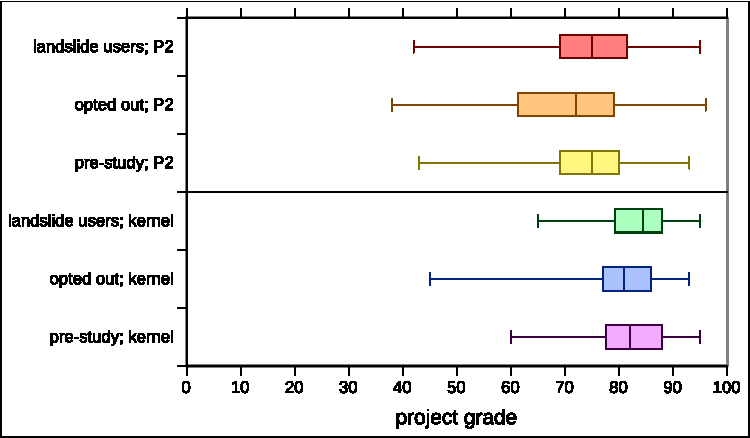
\includegraphics[width=0.96\textwidth]{photo-of-ze-studence.pdf}
		\\
		(a) Visualized as a box plot.
		\\
		\\
		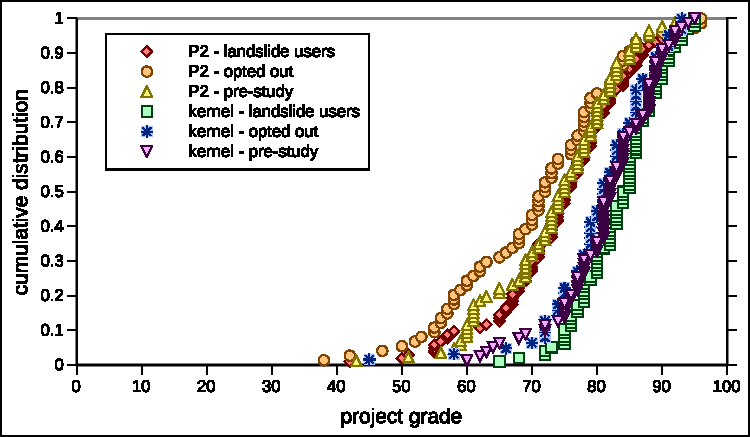
\includegraphics[width=0.96\textwidth]{photo-of-ze-studence-cdf.pdf}
		\\
		(b) Visualized as an EDF.
	\end{tabular}
	\end{center}
	\caption[Distribution of project grades among Landslide users and non-users.]
		{Distribution of project grades among Landslide users and non-users.
	Study participants (S'15 to S'18) are the experimental group;
	non-participants (S'15 to S'18)
	and students from semesters predating the study (F'13-F14) are the control groups.
	Compare Landslide users to non-users for within-semester differences,
	or users to pre-study students to mitigate selection bias.}
	\label{fig:photo-of-ze-studence}
\end{figure}

%We see in Figure~\ref{fig:photo-of-ze-studence} that, indeed,
{\bf Results.}
Overall,
Landslide users did indeed receive
slightly better grades overall on their P2 submissions than non-users from the same semesters,
although comparing to the second control group lessens that difference somewhat.
The difference is also less pronounced in both comparisons among P3 grades
(unsurprisingly, as learning lasting lessons about concurrency should be harder than fixing bugs case-by-case),
although the experimental group still maintains a tiny lead.

{\bf Statistical significance.}
Table~\ref{tab:table-of-ze-studence} presents more detailed statistics from these six distributions.
To assess whether the differences are significant,
% discrete == I used "version 2" of the AD metric that R outputs.
I use the $k$-sample discrete Anderson-Darling test \cite{anderson1952,anderson-darling}
provided by the R statistical programming environment \cite{r-lang,r-ksamples},
comparing each control group to its respective Landslide users group.
Anderson-Darling uses a weighted sum-of-squares distance metric to compare two empirical distribution functions (EDFs),
testing if their samples are likely to arise from the same underlying, though unspecified, distribution.%
\footnote{
I choose Anderson-Darling over the simpler Kolmogorov-Smirnov,
which computes only the maximum instantaneous distance between EDFs,
for its better sensitivity both to repeated deviations and to tail differences \cite{beware-kolmogorov-smirnov}.
}
I deem the difference in grade distributions significant when $p < 0.05$%
% FIXME: is this legit?
% should you be using the combined/grouped AD test instead?
\footnote{I choose not to correct for multiplicity among these 4 comparsons \revisionminor{as} I do in the next section
because each tests a different hypothesis.
},
although as in all $p$-value calculations,
this rejects only the null hypothesis,
not alternative hypotheses,
such as ``more skilled students were more likely to sign up to begin with''.
%
Ultimately, only the same-semester comparisons,
\revisionminor{which do not address that alternative hypothesis,
were significant,
while the cross-semester comparisons,
which attempted to do so,
failed to confidently reject even the null hypothesis.}
However, the distribution difference being smaller in P3 than in P2
% TODO: is there a good way to treat this more formally?
% TODO: run a combined A-D test for each of the two control pairs
further suggests, albeit informally,
that the larger impact in P2 is not attributable {\em only} to selection bias,
or else a similar difference should have been observed in the P3 distributions.
Another possible explanation could simply be that the P3 grading critera result in less grade variance overall,
but this pattern is at least consistent with the ``Landslide helps students submit better P2s'' hypothesis.

% P2 vs opt out
% ad.test(c(42,50,51,55,55,55,56,57,57,58,62,63,65,65,65,66,66,67,67,67,67,68,68,68,69,69,69,70,70,70,70,71,71,71,71,71,72,73,73,73,73,73,74,74,74,74,74,75,75,75,75,75,76,76,76,76,77,77,77,77,78,78,78,78,79,79,79,79,79,79,80,80,80,80,81,81,81,82,82,82,82,83,84,84,84,84,85,85,86,86,86,87,87,87,88,89,90,91,92,93,93,93,95),c(38,42,47,50,52,53,55,55,56,56,57,57,58,58,58,59,60,60,61,62,62,63,65,66,67,68,68,68,69,70,70,70,71,71,71,71,72,72,72,73,73,73,74,74,76,76,76,77,77,78,78,78,78,78,79,79,79,80,82,82,83,83,83,84,84,84,85,86,86,88,90,95,96,96))
%               AD  T.AD  asympt. P-value
% version 1: 2.611 2.139          0.04263
% version 2: 2.760 2.334          0.03576

% P2 vs pre study
% ad.test(c(42,50,51,55,55,55,56,57,57,58,62,63,65,65,65,66,66,67,67,67,67,68,68,68,69,69,69,70,70,70,70,71,71,71,71,71,72,73,73,73,73,73,74,74,74,74,74,75,75,75,75,75,76,76,76,76,77,77,77,77,78,78,78,78,79,79,79,79,79,79,80,80,80,80,81,81,81,82,82,82,82,83,84,84,84,84,85,85,86,86,86,87,87,87,88,89,90,91,92,93,93,93,95),c(43,51,56,58,59,59,60,60,60,60,61,61,61,61,61,62,63,65,65,67,68,69,69,69,69,69,70,70,71,71,72,72,72,73,73,73,73,73,74,74,74,74,75,75,75,75,76,76,77,77,77,77,78,78,78,78,79,79,79,80,80,80,80,80,80,81,81,82,82,82,82,83,83,83,83,85,85,85,86,86,86,88,88,90,92,93))
%                AD    T.AD  asympt. P-value
% version 1: 0.6248 -0.4977           0.6275
% version 2: 0.5790 -0.5581           0.6706

% P3 vs opt out
% ad.test(c(65,68,72,72,73,75,75,75,75,75,76,76,76,76,77,77,77,78,78,78,78,78,78,79,79,80,80,80,80,80,80,80,81,82,82,82,82,82,82,83,83,83,83,83,83,84,84,84,84,85,85,85,85,85,85,85,85,85,85,86,86,86,86,86,86,86,86,86,87,87,87,88,88,88,88,88,89,89,89,89,90,90,90,90,90,91,91,91,91,92,92,93,93,93,94,95,95,95),c(45,58,66,70,72,72,72,72,74,74,74,75,75,75,77,77,77,78,78,78,79,79,79,79,79,79,80,80,81,81,81,81,81,82,82,83,83,83,83,83,84,84,85,85,86,86,86,86,86,86,87,87,89,89,89,89,90,91,91,91,93,93,93))
%               AD  T.AD  asympt. P-value
% version 1: 2.645 2.186          0.04085
% version 2: 2.800 2.398          0.03376

% P3 vs pre-study
% ad.test(c(65,68,72,72,73,75,75,75,75,75,76,76,76,76,77,77,77,78,78,78,78,78,78,79,79,80,80,80,80,80,80,80,81,82,82,82,82,82,82,83,83,83,83,83,83,84,84,84,84,85,85,85,85,85,85,85,85,85,85,86,86,86,86,86,86,86,86,86,87,87,87,88,88,88,88,88,89,89,89,89,90,90,90,90,90,91,91,91,91,92,92,93,93,93,94,95,95,95),c(60,62,63,64,65,68,69,72,72,74,75,75,75,75,76,76,77,77,77,77,78,78,78,78,79,80,80,80,81,81,81,81,81,81,81,81,81,82,82,82,82,82,83,83,83,84,84,84,84,84,84,84,85,86,86,87,87,88,88,88,88,88,88,88,89,89,89,89,89,90,90,90,91,92,92,92,93,94,95))
%               AD   T.AD  asympt. P-value
% version 1: 1.552 0.7322           0.1633
% version 2: 1.640 0.8473           0.1454

% TODO: should i report the T.AD test statistic? i don't even know what it means lol but it's what the p value like, applies to..
\begin{figure}[t]
	\begin{center}
		\small
	\begin{tabular}{cr|r||r|r|r|r||cc}
		\multicolumn{3}{c||}{\bf Population} & \multicolumn{4}{c||}{\bf Distribution} & \multicolumn{2}{c}{\bf Significance} \\
		\bf project & \bf group & $N$ & \bf min & \bf mean & \bf max & \bf stddev & \bf $p$ vs users & \bf cutoff\\
		\hline
			& users		& 103	& 42	& 74.8	& 95	& 10.3	& --	& --	\\
		P2	& non-users	& 74	& 38	& 70.9	& 96	& 12.5	& 0.036	& 0.05	\\
			& pre-study	& 86	& 43	& 73.7	& 93	& 9.7	& 0.671	& 0.05	\\
			\hline
			& users		& 98	& 65	& 83.6	& 95	& 6.2	& --	& --	\\
		P3	& non-users	& 63	& 45	& 80.7	& 93	& 8.2	& 0.034	& 0.05	\\
			& pre-study	& 79	& 60	& 81.6	& 95	& 7.6	& 0.145	& 0.05	\\
	\end{tabular}
	\end{center}
	\caption{Detailed statistics from student grade distributions.}
	\label{tab:table-of-ze-studence}
\end{figure}

% combined test
% > ad.test.combined(list(c(42,50,51,55,55,55,56,57,57,58,62,63,65,65,65,66,66,67,67,67,67,68,68,68,69,69,69,70,70,70,70,71,71,71,71,71,72,73,73,73,73,73,74,74,74,74,74,75,75,75,75,75,76,76,76,76,77,77,77,77,78,78,78,78,79,79,79,79,79,79,80,80,80,80,81,81,81,82,82,82,82,83,84,84,84,84,85,85,86,86,86,87,87,87,88,89,90,91,92,93,93,93,95),c(43,51,56,58,59,59,60,60,60,60,61,61,61,61,61,62,63,65,65,67,68,69,69,69,69,69,70,70,71,71,72,72,72,73,73,73,73,73,74,74,74,74,75,75,75,75,76,76,77,77,77,77,78,78,78,78,79,79,79,80,80,80,80,80,80,81,81,82,82,82,82,83,83,83,83,85,85,85,86,86,86,88,88,90,92,93)), list(c(65,68,72,72,73,75,75,75,75,75,76,76,76,76,77,77,77,78,78,78,78,78,78,79,79,80,80,80,80,80,80,80,81,82,82,82,82,82,82,83,83,83,83,83,83,84,84,84,84,85,85,85,85,85,85,85,85,85,85,86,86,86,86,86,86,86,86,86,87,87,87,88,88,88,88,88,89,89,89,89,90,90,90,90,90,91,91,91,91,92,92,93,93,93,94,95,95,95),c(60,62,63,64,65,68,69,72,72,74,75,75,75,75,76,76,77,77,77,77,78,78,78,78,79,80,80,80,81,81,81,81,81,81,81,81,81,82,82,82,82,82,83,83,83,84,84,84,84,84,84,84,85,86,86,87,87,88,88,88,88,88,88,88,89,89,89,89,89,90,90,90,91,92,92,92,93,94,95)))
%            AD.comb T.comb  asympt. P-value
% version 1:   2.176 0.1655           0.3324
% version 2:   2.219 0.2055           0.3191
%
% > ad.test.combined(list(c(42,50,51,55,55,55,56,57,57,58,62,63,65,65,65,66,66,67,67,67,67,68,68,68,69,69,69,70,70,70,70,71,71,71,71,71,72,73,73,73,73,73,74,74,74,74,74,75,75,75,75,75,76,76,76,76,77,77,77,77,78,78,78,78,79,79,79,79,79,79,80,80,80,80,81,81,81,82,82,82,82,83,84,84,84,84,85,85,86,86,86,87,87,87,88,89,90,91,92,93,93,93,95),c(38,42,47,50,52,53,55,55,56,56,57,57,58,58,58,59,60,60,61,62,62,63,65,66,67,68,68,68,69,70,70,70,71,71,71,71,72,72,72,73,73,73,74,74,76,76,76,77,77,78,78,78,78,78,79,79,79,80,82,82,83,83,83,84,84,84,85,86,86,88,90,95,96,96)),list(c(65,68,72,72,73,75,75,75,75,75,76,76,76,76,77,77,77,78,78,78,78,78,78,79,79,80,80,80,80,80,80,80,81,82,82,82,82,82,82,83,83,83,83,83,83,84,84,84,84,85,85,85,85,85,85,85,85,85,85,86,86,86,86,86,86,86,86,86,87,87,87,88,88,88,88,88,89,89,89,89,90,90,90,90,90,91,91,91,91,92,92,93,93,93,94,95,95,95),c(45,58,66,70,72,72,72,72,74,74,74,75,75,75,77,77,77,78,78,78,79,79,79,79,79,79,80,80,81,81,81,81,81,82,82,83,83,83,83,83,84,84,85,85,86,86,86,86,86,86,87,87,89,89,89,89,90,91,91,91,93,93,93)))
%            AD.comb T.comb  asympt. P-value
% version 1:   5.256  3.058          0.01503
% version 2:   5.560  3.343          0.01109


\subsubsection{Common bugs}
\label{sec:education-eval-bug-case-study}

Based on the results from \sect{\ref{sec:education-eval-bugfinding}},
I selected 4 bugs to study in depth to ascertain
whether Landslide played an instrumental difference
in helping the students ultimately submit respectively correct implementations.
To avoid bias of picking too obscure and/or trivial bugs
that Landslide alone might find but even course staff would not expect students to solve,
I chose only bugs which had substantial penalties in the grading rubric
(guided, as well, by my own intuition as a former TA).
While checking for a given bug's presence by manual inspection,
I blinded myself to whether each group had been a Landslide user or not.
After unblinding, I then re-classified students who used Landslide in general,
but whose usage snapshots showed they did not run the test case in question,
as non-users.
Table~\ref{tab:eval-common-bugs} presents the results.

% TODO check figure placement
\begin{table}[t]
	\begin{center}
		\small
		% note, smth like fisher's method which "combines independent studies into a meta p value"
		% cannot be applied for 2 reasons - 1, these are not independent since the same studence were
		% running landslide on diff test cases; 2, the hypotheses tested are different for each test
	\begin{tabular}{r||cc|cc|c|cc}
		& \multicolumn{2}{c|}{\bf Landslide users} & \multicolumn{2}{c|}{\bf Non-users} & & \multicolumn{2}{c}{\bf Significance} \\
		\bf Bug name & \bf \#correct & \bf \#buggy & \bf \#correct & \bf \#buggy & \bf $\Delta$\%correct & $p$ & \bf cutoff \\
		\hline
		% calculated in R with (rest done similarly)
		% fisher.test(rbind(c(11,10),c(0,16)))$p.value --> 0.0006143355
		Exit UAF  & 11	& 10	& 0	& 16	& $+52.4\%$	& 0.00061	& 0.0125 \\
		% I spent more hours than I should have looking at this landslide-user-submitted-bug group.
		% Can't name the group here, but if you're me and have the analysis file,
		% it's the one from f17 with 3 mutex_test logs in their "u" snapshot.
		% It seems like a mysterious older version of mutex.c was present between their "a" version
		% (which gets fully verified very quickly btw) and their "u" version (for which landslide finds
		% the bug in just a few minutes, no way they could be running the same version; plus the reported
		% data races and so on in the id-log don't line up to the "u" mutex.c source code).
		% That version was correct, then they updated it (introducing the bug) and ran a bunch of other tests,
		% but didn't rerun mutex_test to check their update.
		Mutex     & 17	& 1	& 19	& 0	& $-05.6\%$	& 0.49 & 0.0125 \\
		Paraguay  & 20	& 1	& 14	& 2	& $+07.7\%$	& 0.57	& 0.0125 \\
		% nb this is any downgrade related ding not just dgr tested ones
		% nb 1 is msising bc didn't impl rwlock at all
		% nice p value
		Downgrade & 10	& 3	& 19	& 4	& $-05.7\%$	& 0.69	& 0.0125 \\ % TODO verify these buggers by eye
		\hline
		\bf Total & 58	& 15	& 52	& 22	& $+09.2\%$	& 0.26 & 0.05 \\
	\end{tabular}
	\end{center}
	\caption[Correlation of student Landslide use with solving certain bugs.]
		{
		Correlation of student Landslide use with solving certain bugs in their final submission during Fall 2017 and Spring 2018 semesters.
		%$\Delta P$ stands for the increased probability that a student submits a correct P2
		%(with respect to each bug)
		%given that they use Landslide, versus not using Landslide; i.e.,
		%$P(\mathsf{correct}|\mathsf{landslide})-
		%P(\mathsf{correct}|\mathsf{non\text{-}user})$.
		Note that the totals in the bottom row double-count students,
		which makes sense only if you believe the incidences of each bug in a given submission are independent.
		}
	\label{tab:eval-common-bugs}
\end{table}

Each of the four bugs studied is described in detail as follows.

\begin{enumerate}
\item
{\bf Thread exit/join.}
%During {\tt thr\_exit()}, a thread must arrange for its own stack memory allocation to be freed.
After a thread finishes exiting, the memory allocated for its stack must be reclaimed for other uses.
A common student pitfall is to allow a {\tt thr\_join()}ing thread to free said stack space
while {\tt thr\_exit()} is still executing userspace C code (which typically accesses the stack),
or even for {\tt thr\_exit()} to free it itself.
In the former case, threads must interleave specifically to exhibit a use-after-free;
in the latter case, the use-after-free will be deterministic (i.e., present in all interleavings).
Other than Landslide, however,
the students have no Valgrind-like heap debugging tool which would report a bug immediately upon any illegal heap access.
This means that a subsequent {\tt thr\_create()} invocation would need to race to recycle the memory for a new thread stack
and conflict with the old exiting thread
before any problem could be detected.
The Landslide-friendly test {\tt thr\_exit\_join} is most likely to expose this bug.
%, and
%the official rubric penalties for it are
%{\tt :exit\_stack\_minor -2} and
%{\tt :exit\_stack\_race -4} (for the former case),
%and
%{\tt :uses\_freed\_stack -4} (for the latter).
Whether each student's submitted P2 solved or suffered from this bug
was determined by me personally inspecting their code.
%

\item
{\bf Mutex.}
The Landslide-friendly {\tt mutex\_test} checks for the possibility of two contending threads
accessing a mutex-protected critical section simultaneously.
It includes one thread repeating once the lock, unlock cycle
\revisionminor{(i.e., one contender calls {\tt critical\_section()} twice)}
so as to check for unlock/lock races as well as lock/lock interactions,
and, as mentioned previously (\sect{\ref{sec:education-pebbles-tests}}),
checks for data race access pairs inside the mutex implementation itself.
As students have free rein to design their mutex internals,
this
%refers to
\revisionminor{test probes}
the general class of mutex bugs
in which any number of things can go wrong, depending on the implementation,
leading to mutual exclusion (or otherwise assertion) failure.
Whether each student's submitted P2 solved or suffered from such bugs
was determined by checking their grade files for any mutex-related penalties (assessed by the TAs),
then me double-checking their implementations by hand to confirm.

Further investigating the one group who submitted a buggy mutex,
I found that while they had run {\tt mutex\_test} in Landslide
(and even found and fixed a separate deterministic bug already),
Landslide found no bug in what was presumably a correct implementation,
then they updated % oops
their code, introducing the bug, without testing it again thereafter.
% TODO: some reference to future work about focused testing on small code diffs? talked with some industry ppl about this sometimes

\item
{\bf Paraguay.}
Named after Ivan Jager, the Paraguayan 15-410 TA from 2004-2006 who originally discovered it,
this refers to a condition-variable bug in which a thread which sequentially sleeps on two different condition variables
can spuriously wake up early from the second {\tt cond\_wait()}.
The precise reasoning why many na\"ive student implementations are susceptible to this bug,
as well as the 3 major ways of fixing it,
are one of 15-410 staff's closely-guarded secrets (\sect{\ref{sec:410-secrecy}}).
Suffice it to say that the {\tt paraguay} test invokes a custom Pathos {\tt misbehave} mode
which biases thread scheduling towards the interleaving required to exhibit the bug
(Landslide, of course, replaces this {\tt misbehav}iour with model checking).
% TODO: i feel tihs sentence should go somewhere else, like after analysis, not in description
Hence, despite being a subtle concurrency bug,
the official course test suite is likely to expose it,
so comparing how many Landslide users and non-users submitted this bug in particular
would speak more to the impact of Landslide's preemption traces
in helping to diagnose a bug that a ``stress'' test could already find.
%
{\tt paraguay} is itself the Landslide-friendly test for its eponymous bug.
%, and
%the official rubric penalty for it is
%{\tt :paraguay -2}.
Whether each student's submitted P2 solved or suffered from this bug
was determined by me personally inspecting their code.

\item
{\bf R/W-lock downgrade.}
In addition to the standard R/W-lock interface,
P2 requires students to implement {\tt rwlock\_downgrade()}:
called with the lock held in write mode,
the caller adopts the reader role instead,
allowing other waiting reader threads to proceed simultaneously,
all while allowing no waiting writers to access in between.
%
The Landslide-friendly test {\tt rwlock\_downgrade\_read\_test}
checks that readers are allowed simultaneous access after a downgrade with no possibility for deadlock.
Rather than one specific bug, this refers to any of several failures that can arise during a downgrade.
%, and
%the official rubric penalties related to this bug are
%{\tt :downgrade\_no\_signal -1},
%%{\tt :unsafe\_rwlock\_downgrade -2}, % don't think this is right; not relevant anyway (overlaps)
%{\tt :downgrade\_partial\_signal -1}, % not sure if this means smth that dgr would expose
%{\tt :downgrade\_\allowbreak{}lies -3}, and
%{\tt :downgrade\_deadlock -4}.
Whether each student's submitted P2 solved or suffered from these bugs
was determined by checking their grade files for any downgrade-related penalties
(which were assessed by the TAs as a result of their manual inspection, rather than mine).
\end{enumerate}

{\bf Statistical significance.}
% two-tailed btw, the better (more conservative) way,
% tbh one tailed might even make sense here, but it doesn't change anything wrt the cutoffs anyway, so
The $p$ values
in Table~\ref{tab:eval-common-bugs}
are calculated in R \cite{r-lang} using Fisher's exact test \cite{fishers-exact-test},
treating each row as an independent 2x2 contingency table.
I divide 0.05, the standard significance cutoff,
by the number of bugs to conservatively account for multiplicity \cite{xkcd-jellybeans}
(not that it matters with these $p$ values).

The latter three bugs' occurences are thoroughly uncorrelated with Landslide use,
the {\tt thr\_exit()} bug standing alone with extremely high significance:
not a single student who did not use Landslide these semesters
submitted a correct implementation.
This difference is easily explainable:
the class-provided unit tests already do a good enough job catching the other three bugs
that students are able to find and fix them before submission regardless of what testing tool they used.
(The high correct-to-buggy ratio corroborates this.)
Nevertheless, that does not mean Landslide is pointless for these bugs;
it may well have helped the students reproduce them more reliably and/or diagnose them faster.
This is merely a null result for submission quality, not necessarily a negative one,
and the next section will attempt to evaluate such quality-of-life improvements instead.

On the other hand, because the {\tt thr\_exit()} bug typically manifests as a use-after-free,
the official tests must stress the thread library until the memory in question gets re-allocated
in just the right interleaving pattern to cause corruption that leads to a visible crash.
Landslide, meanwhile, detects this error immediately upon access (\sect{\ref{sec:landslide-valgrind-mode}}),
with no need for complex corruption conditions.
Among the 11 Landslide users who submitted correct {\tt thr\_exit()}s in this regard,
it is difficult to say whether the heap checking alone, together with unit or stress tests,
would have been sufficient,
or whether heap checking and model checking were both necessary in concert to help them.
To isolate the impact of model checking,
I simulated the students having access to a stand-alone heap checker
by checking only the first thread interleaving with Landslide
% TODO - more specific section reference - quicksand det/nondet drpps eval
(similarly to \sect{\ref{sec:quicksand-eval}})
and assuming the students would find and fix any such ``deterministic'' use-after-free bugs before the deadline.
Re-classifying these into the ``correct'' group,
the 11-10-0-16 distribution becomes
% fisher.test(rbind(c(11,10),c(3,13)))$p.value -->  0.0475343
11-10-3-13,
with a new $p$ value of 0.048:
still positively correlated, but no longer significant under the multiplicity-corrected cutoff.

\subsection{Survey responses}
\label{sec:education-eval-survey}

Analyzing only the raw technical data of how users interacted with Landslide can paint only part of the picture.
For one, offering students better testing and debugging tools
may not necessarily find strictly more bugs or help students submit more correct implementations
than with stress testing;
it may instead find the same bugs faster,
affording the students more free time apart from the project,
a quality-of-life improvement normally invisible to graders.
For \revisionminor{another}, Landslide's automatic snapshots, being captured at the time of issuing each preemption trace,
necessarily miss the student's subsequent experience interpreting them.
The surveys listed in sections \sect{\ref{sec:education-survey-pebbles}} and \sect{\ref{sec:education-survey-pintos}}
serve to probe these more qualitative aspects of the Landslide experience.

\begin{figure}[p]
	\begin{center}
		\begin{tabular}{cc}
			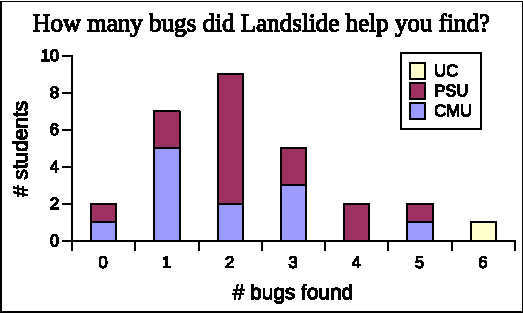
\includegraphics[width=0.42\textwidth]{survey1.pdf} &
			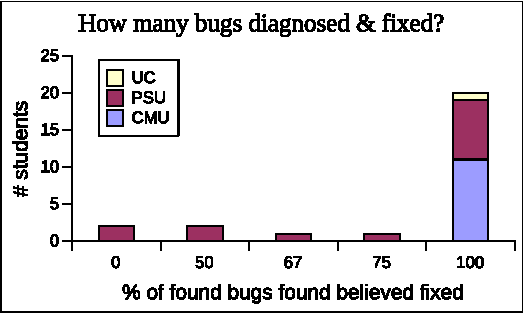
\includegraphics[width=0.42\textwidth]{survey2.pdf} \\
			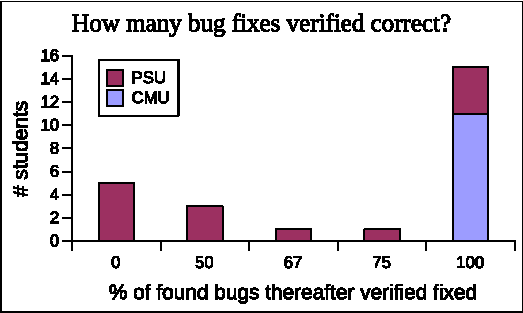
\includegraphics[width=0.42\textwidth]{survey3.pdf} &
			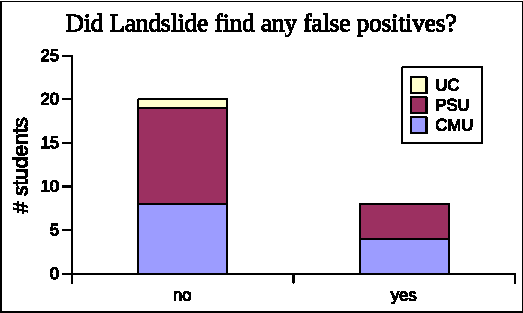
\includegraphics[width=0.42\textwidth]{survey4.pdf} \\
			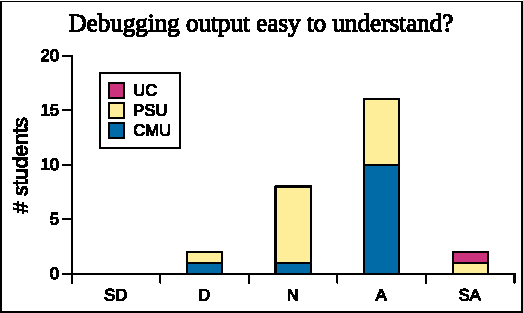
\includegraphics[width=0.42\textwidth]{survey5.pdf} &
			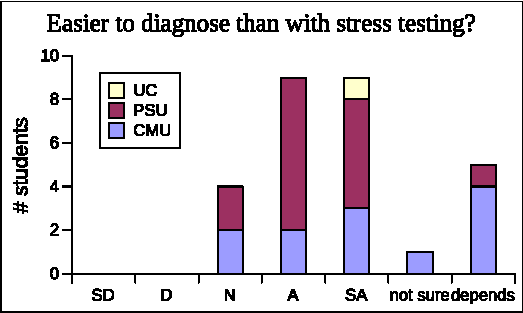
\includegraphics[width=0.42\textwidth]{survey6.pdf} \\
			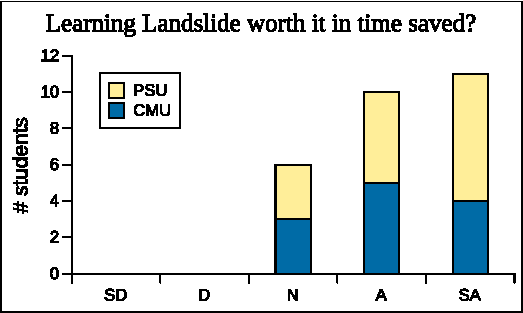
\includegraphics[width=0.42\textwidth]{survey7.pdf} &
			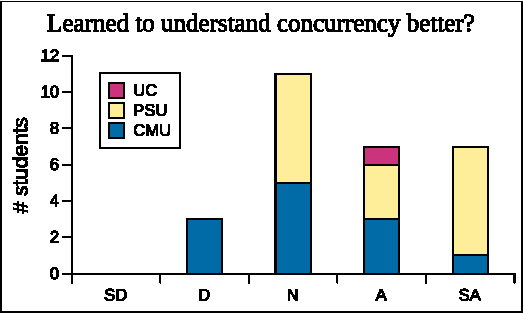
\includegraphics[width=0.42\textwidth]{survey8.pdf} \\
			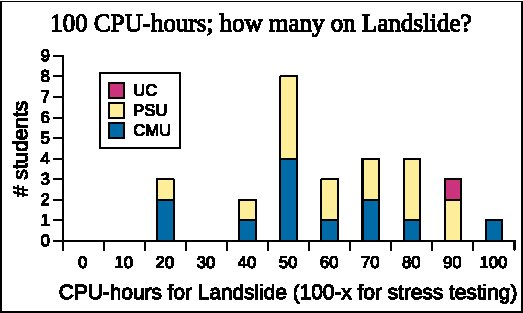
\includegraphics[width=0.42\textwidth]{survey9.pdf} &
			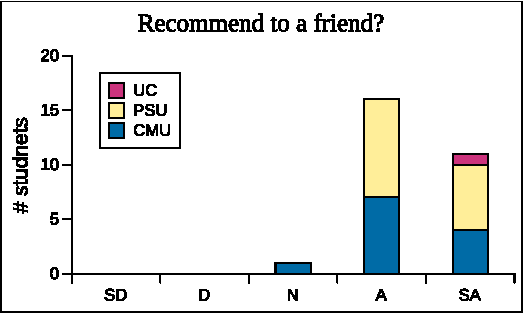
\includegraphics[width=0.42\textwidth]{survey10.pdf} \\
		\end{tabular}
	\end{center}
	\caption[Student survey responses.]
		{Student survey responses.
	SD/D/N/A/SA stands for
	strongly disagree/\allowbreak{}disagree/\allowbreak{}neutral/\allowbreak{}agree/\allowbreak{}strongly agree.}
	\label{fig:survey}
\end{figure}

\subsubsection{Response data}
\label{sec:education-survey-response-data}

% probably just better to state this in one line of prose
%\begin{table}[h]
%	\begin{center}
%		\begin{tabular}{r|crcrc|r}
%			& \multicolumn{5}{c|}{\bf Did survey?} & \\
%			\bf Semester & & \bf yes & & \bf no & & \bf Total \\
%			\hline
%			CMU F'17	& &  7 & &  7 & & 14 \\
%			U. Chicago F'17	& &  1 & &  3 & &  4 \\
%			CMU S'18	& &  5 & &  5 & & 10 \\
%			PSU S'18	& & 11 & & 27 & & 38 \\
%		\end{tabular}
%	\end{center}
%	\caption{Survey response rate among students who used Landslide. (The survey was first introduced in F'17.)}
%	\label{tab:photo-of-ze-surveys}
%\end{table}

The response distributions for each of the surveys' multiple choice questions
are shown in Figure~\ref{fig:survey}.
In total, 28 students (or pairs thereof) answered the survey:
12 pairs from CMU, 15 individuals from PSU, and 1 pair from U. Chicago.
The first four questions/graphs focus on concrete debugging results,
and the latter six on the students' subjective opinions.
%
Note that two of the questions
(3 and 7 from \sect{\ref{sec:education-survey-pebbles}})
were not asked on U. Chicago's version of the survey,
so their corresponding graphs show only CMU and PSU response data.
Likewise, U. Chicago's questions 4, 8, and 10
(see \sect{\ref{sec:education-survey-pintos}}),
which were not asked on CMU's and PSU's surveys,
having only one respondent,
are not pictured;
the answers thereto were ``15-20 minutes'', ``Agree'', and ``Agree'', respectively.
Also, this respondent's answer of 6 on the ``How many bugs'' question
appears to indicate the total number of preemption trace files course staff sent them;
%despite the attached ``some of these may indicate the same bug'' disclaimer;
upon further investigation,
the 6 traces seem to represent 2 distinct bugs among them (\sect{\ref{sec:education-eval-bugs-uc}}).

The survey responses were very positive:
% TODO: corroborate this with snapshot data?
students reported being able both to diagnose and to verify as fixed the vast majority of Landslide's reported bugs,
compared Landslide favorably to stress testing,
and found the experience worthwhile and worth recommending.
Regarding the 100 CPU-hours question in particular,
students could approach answering it in several different ways:
do the three students who answered 20/80 think stress testing is four times as good as Landslide at finding bugs,
or that stress testing requires four times as long to reach the same point of diminishing returns?
On the other extreme, one student said they would spend all 100 CPU-hours on Landslide,
which probably speaks more to their enthusiasm than to a careful attempt to maximize expected number of bugs found
% TODO: put a section reference to future work resource exhaustion / malloc failure injection discussion
(even the author themself recognizes stress testing's advantages for certain types of bugs, such as resource exhaustion).
Nevertheless, the responses' overall bias to spending at least half the CPU-time on Landslide
shows clearly that the students found the experience worthwhile.

Three questions with open-form answers bear further discussion:
what kind of false positives Landslide reported, % oopsative mood
reasons they found it worth recommending to a friend,
and suggestions for improving the interface
(PSU only\footnote{I thought to ask this question too late for CMU's surveys.}). % ososugichatte

\subsubsection{False positives}
\label{sec:education-eval-survey-falsepositives}

Even though 71\% of students reported receiving no false positive bug reports,
the nature of Landslide's bug-detection algorithms is such
that it should ideally never report any correct behaviour as wrong,
so I consider those 29\% that did report such the most negative result among the survey responses.
They described their false positives, and I either make excuses or own up, as appropriate, as follows.
Reports from CMU students (Simics version):
\begin{enumerate}
	\item Landslide complained of a nonexistent {\tt MAGIC\_BREAK} (\revisionminor{a} Simics debugging function),
		despite the student's code never invoking it.
		This arose because of technical confusion between the test program's and the shell's address spaces,
		and was subsequently fixed in commit 3f24d67 (Simics repository only).
	\item Landslide reported ``some weird errors'' and/or mysteriously crashed
		when multiple instances were run from the same directory.
		(Multiple students suffering this failure mode contacted me for support,
		though only one reported it on the survey;
		in some cases, I recall said weird errors manifesting as false positive invalid heap access reports.)
		Simultaneous Landslides can clobber certain auto-generated header and/or temporary files,
		scrambling its instrumentation and leading to chaotic behaviour.
		I introduced a guard against this in commit 977e8fb (Simics repository) and e49b5df (Bochs repository).
	\item One student reported ``Data races which I believe they are not''.
		Looking at their usage snapshots to corroborate this,
		these appear to be true, yet benign, data races
		(in several cases corresponding to {\tt mutex\_test}'s verification of the mutex's internal memory accesses
		(see \sect{\ref{sec:education-pebbles-tests}}));
		i.e., expected behaviour rather than false positive bug reports.
		Student confusion about these could be alleviated
		by improving Landslide's user interface messages when printing data race information. % uuuuuuu its already so
	\item One student complained of a bug report that, while truly a bug, showed wrong filenames and line numbers in stack traces,
		and (quite naturally) suggested that accurate stack traces would make debugging easier.
		Checking against their usage snapshots,
		this seems to be an issue with Simics's symtable's handling of assembly functions.
		The Bochs version handles these correctly.
\suspend{enumerate}
Reports from PSU students (Bochs version):
\resume{enumerate}
	\item Landslide kept crashing for one student while running {\tt paraguay}.
		This is likely due to exceeding Linux's process limit and/or exhausting the class's official VM's memory,
		which can arise when many data race candidates cause Quicksand to spawn many Landslide jobs,
		and (as on {\tt paraguay}) each with very large state spaces that must defer.
		I had been working on mitigating this problem just before beginning the PSU study;
		properly addressing it would involve improving Quicksand's memory-exhaustion detection code
		and/or making Quicksand at all aware of the process limit to begin with.
		(Note that this is not strictly a false positive bug report, just a Landslide crash.)
	\item Students who initialized child threads with a base pointer value of {\tt 0xffffffff} observed Landslide crashes,
		as it attempted to stack trace through that address and access memory that wrapped around the address space.
		(Several students contacted me about this via email, and I issued a prompt fix;
		one student later reported it on the survey.)
		Commits 0573e34 (Bochs repository) and 654f459 (Simics repository) fixed this bug.
		(\revisionminor{As} above, not actually a false positive bug report.)
	\item Landslide issued false invalid heap access reports to one student
		who had been using {\tt new\_pages} to allocate thread stacks ``very close'' to the {\tt malloc} heap.
		They reported this during the study and I fixed it promptly for them in commit 4a26da7 (Bochs repository only),
		then reminded me of it again in the survey.
	\item Finally, one student reported simply, ``Race condition''.
		Without the same usage snapshots to consult as I'd have for a CMU student,
		or more self-reported detail, I regrettably can offer no comment.
\end{enumerate}

\noindent
Overall, most of the issues reported as answers to the ``false positive'' survey question
were merely Landslide crashes or user interface confusion.
Those few truly erroneous bug reports (items 1, 2, and 7),
while certainly guilty of burdening % oopsative mood
students with worry over whether the problem is their own code or in Landslide itself,
are at least not too discouraging for two reasons.
Firstly, in all cases the students were able to recognize the false positive quickly enough to ask for help,
and I was able to deploy a fix and let them proceed before the project came due.
Secondly, each such problem, now having been fixed, will befall no future student again --
not to assert Landslide is completely bug-free now,
but at least that it grows more and more stable with each passing semester.

\subsubsection{Reasons worthwhile}

After
%the question
asking ``Would you recommend a friend taking OS next semester to use Landslide?'',
I asked the students for open-form reasons why or why not.
As the former question's answers were exclusively positive (only 1 student even answering ``no opinion''),
this question's answers turned out to be mostly praise.
\revisionminor{Three} students declined to answer this question;
I reproduce the rest here, paraphrasing for clarity and brevity,
\revisionminor{denoting my own clarifications and commentary with [square brackets]}.%
\footnote{Note that most students used the term ``race condition'' rather than ``concurrency bug'',
as taught in CMU and PSU lecture material;
I replaced these while paraphrasing in accordance with \sect{\ref{sec:glossary}}.}
Answers from CMU:

\begin{enumerate}
	\item Easy to use and found nontrivial bugs.
	\item Useful to find some bugs, but other types of bugs (such as memory corruption) were impossible to find with Landslide.
	\item Helped verify our atomic primitives were correct.
	\item Would recommend, but takes too much time [unclear, but seems to be referring to execution time rather than setup/usage].
	\item Tests are automated and can be left running for a long time.
		However, faced uptime issues with CMU's Linux servers (which reboot every night);
		wished for a more reliable execution environment.
	\item It's pretty helpful. % lol
	\item Seems more reliable than stress tests.
	\item Found a bug not found by stress tests.
	\item Finds concurrency bugs with little effort that may be undiscovered otherwise.
		[This respondent also provided some interface feedback here, since I didn't ask CMU students a separate question for such;
		see next section.]
	\item Easy to learn and a simple way to test our P2.
\suspend{enumerate}
Answers from PSU:
\resume{enumerate}
	\item Although didn't find any concurrency bugs for me, gives me more confidence about my code.
	\item Helpful, just didn't have a lot of time to use it.
	\item Does not make concurrency debugging easy, but definitely makes it easier.
	\item Helpful to find bugs you weren't previously aware of.
		Makes more sense to use an expressly designed tool rather than [unit/stress] tests
		\revisionminor{which may or may not find bugs}.
	\item Helpful and easy to use.
	\item Saves time overall, can run long tests overnight.
	\item Helps to find concurrency bugs and their root causes better than stress tests.
	\item It finds the concurrency bugs you need to fix for full credit.
	\item Helpful for finding some uncommon bugs I hadn't found or wasn't looking for.
	\item Found bugs I kept overlooking, which may have taken many hours to find otherwise.
	\item Helpful for the difficult step from code being ``finished''
		[scare-quotes theirs; presumably meaning ``feature-complete'']
		to getting rid of all concurrency bugs.
	\item Easy to use, setup taking no more than 5-10 minutes, and allowing being run overnight.
	\item Very efficient at concurrency testing.
		Stress test crash reports do not necessarily point to the root cause, due to memory corruption for example;
		plus bugs may not show up every time due to nondeterminism.
	\item Helped find a bug I wouldn't have found otherwise.
		Did not show an interleaving directly [i.e., did not issue a bug report],
		but reported a data race that turned out to be a concurrency bug upon inspection.
\suspend{enumerate}
Answer from U. Chicago:
\resume{enumerate}
	\item Found several subtle, legitimate bugs we wouldn't have easily caught otherwise, but made sense once revealed.
		Fixing them took little time but allowed us to proceed confidently on the next project.
		Often wished for Landslide to have been available to use during the next project as well.
\end{enumerate}

\noindent
Overall, students most commonly praised Landslide's ease of use,
its ability to find bugs that elude stress testing,
and the confidence instilled from verifying bugs had been fixed.

\subsubsection{Interface suggestions}

Lastly, I asked the PSU students for any feedback they might have on making Landslide's interface easier to use or understand.

\begin{enumerate}
	\item Requested for preemption traces to be more clear about the meaning of each stack trace in each table cell,
		and complained of inaccurate line numbers
		[likely referring to how the current behaviour indicates the line of code {\em after} a function call,
		corresponding to the {\tt call} instruction's pushed return address,
		rather than the function call itself]. [This answer from CMU; see above.]
	\item Including a manual or tutorial would be helpful [presumably beyond the user guide's instructions, such as recapping the procedure shown in the lecture demo which wasn't written down anywhere].
	\item Don't print warnings about line length exceeding 80 characters [inconsistency between 15-410 and \psuos compilation options].
	\item ``It takes too long. But I guess that's impossible to fix.'' [Well, it's an open research problem to fix!]
	\item Preemption traces should explicitly indicate where in the interleaving the bug occurred.
		[Root cause identification is its own research area, but more detail is certainly possible.]
	\item Improve explanation of data races [in the user guide, perhaps].
	\item Happy with it as-is [\revisionminor{reported by three} students]
		% wow, latex -- if you put [] outside of the revision, everything is awful forever
	\item \revisionminor{[Seven non-respondents]}
\end{enumerate}

Though I did not ask this question on the CMU survey,
my experience handling student questions in person
suggests CMU students
\revisionminor{(as well as Professor Eckhardt)}
also mostly wish for
better explanations of data races and
more detail and clarity in the preemption traces.
Though I present the formal definition of data races in the lecture
(\sect{\ref{sec:education-pebbles-recruiting}})
and refer back to it in Landslide's documentation and output,
showing a concrete example
in future iterations of the user guide
would go a long way to illustrate the abstract concepts.
The preemption traces could be improved by making it clearer that the stack trace in each cell of the table
represents executing the thread in question from wherever it previously left off (or its inception)
all the way until it reaches that stack trace, then preempting it to run another thread.
They could also easily report more diagnostic information;
for example, showing the sets of memory conflicts between each thread,
annotating the type of each preemption point (yield, mutex, or data race),
and/or indicating the adversarial memory access for each data race preemption point.

\subsubsection{Other universities}

Comparing the survey response distributions between CMU versus PSU and U. Chicago (Figure~\ref{fig:survey}),
CMU students tended to verify their bugfixes more often by re-running Landslide
and found the preemption traces easier to understand,
while PSU and U. Chicago students generally compared Landslide more favourably to stress testing
(CMU students comparatively preferred the more nuanced answer that it depends on the type of bug),
and reported more often that \revisionminor{it} helped them understand concurrency better.
%Considering that CMU's 15-410 demands substantial prerequisite concurrency experience
%(15-213 \cite{csapp} or equivalent)
%whereas PSU's \psuos is more towards the average between CMU's 15-213 and 15-410
%(tempering the difficulty of P2 to make it more accessible (\sect{\ref{sec:overview-psu}})),
Considering the higher demand CMU's 15-410 makes for prerequisite concurrency experience
compared to PSU's relative tempering of P2's difficulty to make it more accessible (\sect{\ref{sec:pebbles}}),
% TODO: represent u c in this sentents?
these trends seem to correlate with the different levels of preparation each course's students had,
showing that students of various skill levels
can each benefit from the experience in different ways.


% TODO

%%%%%%%%%%%%%%%%%%%%%%%%%%%%%%%%%%%%%%%%%%%%%%%%%%%%%%%%%%%%%%%%%%%%%%%%%%%%%%%%

\section{Discussion}
\label{sec:education-discussion}

Human subjects research is inherently messy.
Each of the previous section's approaches to evaluating Landslide's educational value
was accompanied by some drawback which prevented it from being perfectly objective science,
but many of them presented tentatively positive results nonetheless,
\revisionminor{and relatively very little negative feedback such as false positives}.
Landslide helped many students find and fix many bugs (\sect{\ref{sec:education-eval-bugfinding}}),
but making a direct comparison to stress testing, the prior state of the art, is not straightforward.
%and not statistically significant,
Immediate improvement in students' project grades was observed
(\sect{\ref{sec:education-eval-grades}}),
although statistical significance was lost when attempting to account for selection bias;
and impact on grades alone is a very narrow measure of pedagogical value anyway.
Landslide's debugging power was also found to be statistically significant
for the {\tt thr\_exit\_join} bug in particular.
Students responded overwhelmingly positively in the survey (\sect{\ref{sec:education-eval-survey}}),
although it is easy to imagine students being equally happy with a ``debugging tool'' that just tells them all the answers.

Nevertheless, I believe each of these partial results taken together
paint an overall picture of success:
students fixed their own bugs {\em and} were happy about it;
students were able to ask for help rather than be deterred by inevitable technical difficulties as far as I know;
students provided intelligent feedback suggesting they truly understood the debugging process;
% well not the student who said "traces should point to where the bug is" but eh can't win em all c.c
et cetera.
%
The rest of this section will discuss the study's limitations and provide some perspective for the future.

\subsection{Bias}

% TODO - u can verify the bug just by taking survey graph #1 and comparing to landslide snapshots (sep. by groups who answered survey)
% anything else?

As long as an educational user study is run on a volunteer basis,
one cannot completely avoid selection bias:
those with enough free time to participate are more likely to be the most capable students already,
who are least in need of the extra debugging help.
This was especially evident in the annotation-required P3 study from \revisionminor{2012} \cite{landslide},
in which only 5 groups volunteered (15\% of the 34 total who submitted P3 that semester),
among which 2 had enough after just the annotation phase and did not continue to do any in-depth testing.
In contrast, since switching to the automatically-annotatable P2,
the participation rate rose to 58\% (Table~\ref{tab:photo-of-ze-studence})
among all P2-submitting groups.
Reaching over half the class could already be seen as a major step in mitigating said selection bias.

The survey may also be susceptible to several sources of bias beyond participation itself.
I suspected students might feel inclined to be overly polite in their answers
(whether consciously or subconsciously).
I attempted to counteract this by concluding my survey link emails with,
{\em Please try to answer honestly rather than flatteringly--if any part
of the experience was bad for you, I want to hear about it to make
Landslide better in the future!}
It's also possible that survey respondents % respondence
were more likely to be those who enjoyed Landslide the most,
meaning I might not hear as much negative feedback as I should.
% trying to isolate this bias would be pretty fraught...
% possible flaws in table: students who found bugs might have had either a good (bug!) or bad (false positive) experience
% could studence who didn't find bugs also have had a good experience, like enjoying the verification guarantee
% think of how to say it presentably...

% TODO: is this ok to report without IRB approval? ask dave
I took no special measures to compensate for bias in gender, race, or being non-natively English-speaking
during recruitment or the survey.
Surveying students to measure any differences in these demographics between study participants and the overall class population
would have required mandatory survey participation,
and in turn, a more rigorous IRB approval process.
According only to my memory of students who attended the Landslide clinics
(\sect{\ref{sec:education-pebbles-recruiting}}),
the racial diversity was roughly representative of the class at large,
and the proportion of women I perceived was in fact somewhat higher than the overall gender ratio.
More scientific analysis of such statistics was deemed beyond the study's scope for now.

\subsection{Retrospect}

\revisionminor{Aside from} just trying to draw firm conclusions from
the opinions of students who are just learning concurrency to begin with,
student feedback in turn guided the constant development
of Landslide, and the experimental design itself,
as the semesters went by.
In this section I will fantasize about how I might have run more perfect experiments
granted the impossible wish of knowing then what I know now.

\subsubsection{Pebbles}

The survey was introduced into the study only in time for two semesters' worth of student responses,
after several iterations of collecting only usage and bug report snapshots.
Apart from the obvious improvement of having been surveying students from the beginning,
the following questions could have improved the survey.
\begin{enumerate}
	\item {\em Did you have any technical difficulties with Landslide that I had to intervene on,
		whether in person or over email?}
		(Some students reported this in the ``false positives'' question,
		although fewer than I helped overall, so others must have not mentioned it.)
		Comparing answers to this question across subsequent semesters would give a sense
		of how much Landslide's stability was improving over time
		and whether it was mature enough for unsupervised use in the future.
	\item {\em How well do you feel you understood the research challenges explained in the lecture?}
		and,
		{\em How well do you feel a user should need to understand same in order to benefit from Landslide's bug reports?}
		(Answers on a scale from ``Not at all; Landslide is a magic black box to me''
		to ``I'm ready to work on research in this field myself''.)
		These questions would help fine-tune the lecture material and user guide to maximize student comfort,
		and potentially also corroborate the claim that Landslide is accessible even to novice users.
	\item {\em What additional debugging information would you want displayed on the preemption traces?}
		Knowing now that interpreting preemption traces was a sticking point for many users,
		I would hope to identify the most wished-for features to know what to prioritize improving.
		This could also assess students' understanding of what kinds of information
		would or would not be reasonable for Landslide to record and report.
	\item {\em For each bug Landslide found in your code, how trivial or severe do you feel it was?}
		This would help get a sense of how the students regarded Landslide
		on a spectrum between annoying style checker \revisionminor{and} life-saver,
		and potentially suggest options to make Landslide suppress certain types of bug reports.
		For example, it currently reports spin-wait loops in {\tt mutex\_lock()} as bugs
		with a special message referring students to relevant lecture slides,
		but it's possible refusing to test any code beyond until that bug was fixed
		might have made Landslide less useful overall.
	\item \revision{{\em In addition to finding bugs, did you manage to fully verify your code under
		any of the tests by letting Landslide complete all state spaces before reaching the specified time out?}
		This would provide a sense of how thoroughly students understood the underlying research technique,
		and serve as a follow-up to the ``how many bug fixes verified'' question
		(where students often stopped Landslide midway through after a little while).}
\end{enumerate}

Some students (around 0 to 2 per semester if memory serves)
emailed me during P3
to ask if they could test their kernels with Landslide just like their thread libraries.
I answered each by explaining that it would take more effort on their part,
and then, if they were still interested,
guided them through the annotations on a case-by-case basis.
This process was not included in the IRB-approved study protocol,
so I collected no results from them.
If I had planned in advance, I could have supported this ``bonus stage'' officially,
and further surveyed the brave volunteers about how P3 Landslide could be made more generally accessible.

Finally, to evaluate whether the experience of using Landslide
left the students with any lasting lessons learned,
a follow-up survey could have been given one or two years later.
Such a survey would ask, for example,
{\em Have you encountered any debugging problems since finishing OS that made you wish for a tool like Landslide?}
and
{\em Do you feel the way you think about testing, debugging, and program correctness
has been influenced in any way by using Landslide?}
to evaluate its lasting impact on their understanding of concurrency.

\subsubsection{Pintos}

While part of the point of this experimental design was to evaluate Landslide as a grading tool in the hands of TAs,
I would be remiss \revisionminor{not}
to mention that I also feared the automatic annotation process would not be as robust as the P2 version.
Indeed, while helping Kevin get oriented with using Landslide,
I implemented
several
fixes/improvements to the setup scripts
as I found student kernels that failed to automatically annotate
(for example, those with {\tt ready\_list} changed to an array,
as described in \sect{\ref{sec:education-pintos-instrumentation}}).
Had I given Landslide directly to students that semester,
the students themselves would have had to email me for tech support.

I attribute the comparatively low participation rate of Pintos students to two major factors:
one, not incentivizing the students to directly improve their grades
(instead offering only the vague promise of a ``learning experience'' debugging their code after handin),
and two, not traveling to the university to introduce the research topic in an in-person lecture
(leaving the students potentially confused about what advantage, if any, was offered over stress testing).
Hypothetically, I could have achieved greater user study participation
either by \revision{giving a lecture remotely via videoconference},
by offering extra credit to students,
or by offering an autograder-like interface for students to receive bug reports before their deadlines instead of after
(either way requiring a more rigorous IRB review process).

\subsection{Future educational use}

%{\bf Pebbles.}
Now being done collecting student usage data to publish as research results,
and no longer bound by the IRB's requirement that Landslide be isolated from the grading process
lest it be seen as coercion to participate,
Professor Eckhardt and I have discussed options to deploy it as an official part of 15-410's curriculum.
This section has already clearly shown students are capable of debugging with it on their own time,
and I believe it well-automated enough to supplement Fritz (the existing stress testing infrastructure)
in the class's grading process as well.
TAs could also, at their option, use Landslide by hand to confirm any bugs encountered during manual inspection
and/or write new Landslide-friendly tests to expose bugs not yet targeted by the 6 tests offered here.

Over the study's seven semesters,
I believe the stability of Landslide's instrumentation process has improved enough
to require little to no ongoing technical support anymore,
although Landslide-specific office hours may still prove helpful.
I am willing to continue giving the guest lecture as long as proximity and curriculum allow,
although I also hope the documentation herein be enough to pass the mantle like any other piece of the course infrastructure.
Future problems to address include grading bias
(i.e., students submitting blindly-hacked code that just barely passes Landslide,
even if not necessarily correct,
thereby gaming the autograder),
and improving usability to reach even the most struggling students
(i.e., that last 42\% who submitted P2s without participating in the study).

%{\bf Pintos.}
Regarding non-research use in Pintos classes,
Landslide can now handle a considerably wider variety of student implementation quirks
on account of the fixes from this time (\sect{\ref{sec:education-pintos-instrumentation}}).
In its original shape
(before the F'17 semester,
having only enough instrumentation necessary for the Pintoses used in \sect{\ref{sec:quicksand-eval}}'s experiments),
Landslide was already able to automatically instrument 18 out of the 21 {\tt threads} project submissions at U. Chicago.
I was able to quickly deploy a fix to make the annotation scripts handle the other 3 cases,
although such technical support is not something any TA would be able to do.
%
In its current shape I would recommend it for TA use grading,
but not necessarily directly to students without someone familiar with the codebase on immediate hand for tech support.
However, I also believe Landslide's success in these user studies,
provided me present to handle technical issues,
serves as testament for stateless model checking in general in the educational theatre.
While Pintos's kernel-level environment presents a unique challenge for concurrency testing,
other, more readily automatic model checkers for user-space programs,
such as dBug \cite{dbug-ssv} or CHESS \cite{chess},
could easily be used on other thread-library-like programming projects at any university.

